\begin{landscape}
\begin{figure}[p]
\centering
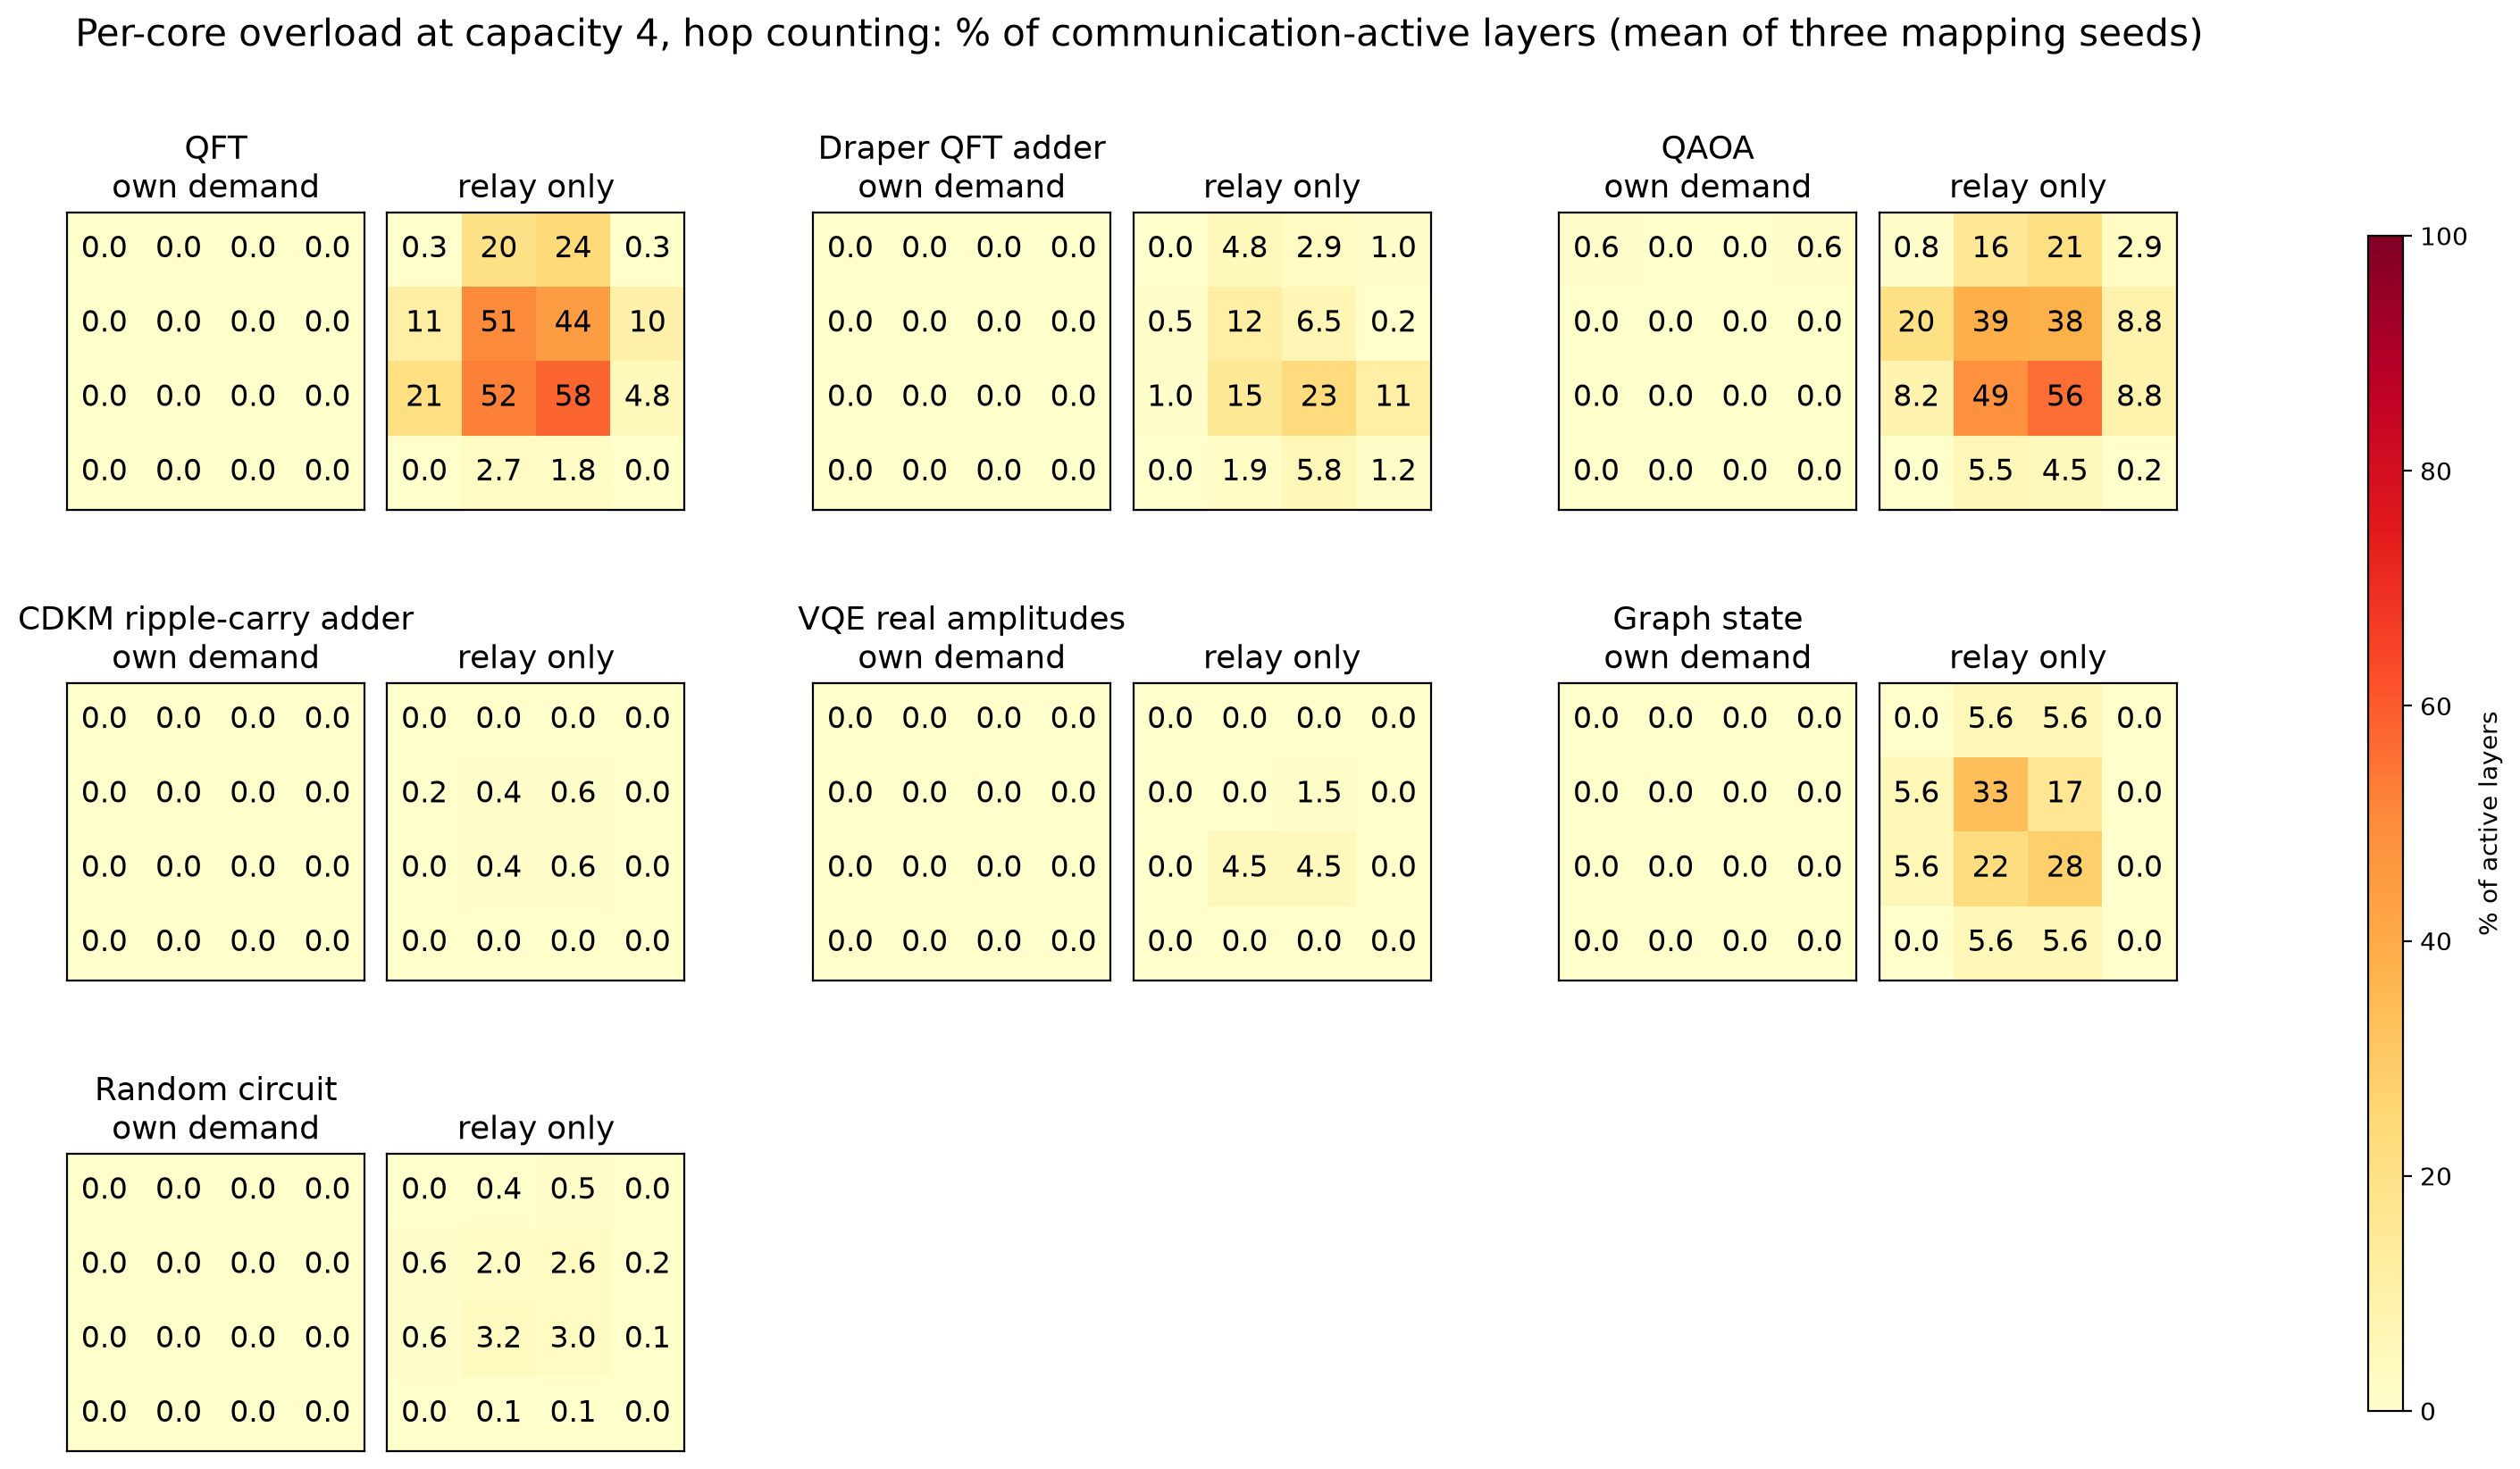
\includegraphics[width=\linewidth,height=0.80\textheight,keepaspectratio]{exp2_overview_c4_hop.png}
\caption{Capacity 4, hop counting. For each workload with overload, the left heatmap is the percentage of its active layers in which the core is overloaded by its own endpoint demand and the right heatmap the percentage in which it is overloaded only because of relay traffic. Mesh cores are numbered row by row (core 10 is row 2, column 2). Mean of three mapping seeds.}
\label{fig:exp2-overview-c4-hop}
\end{figure}
\end{landscape}
\begin{landscape}
\begin{figure}[p]
\centering
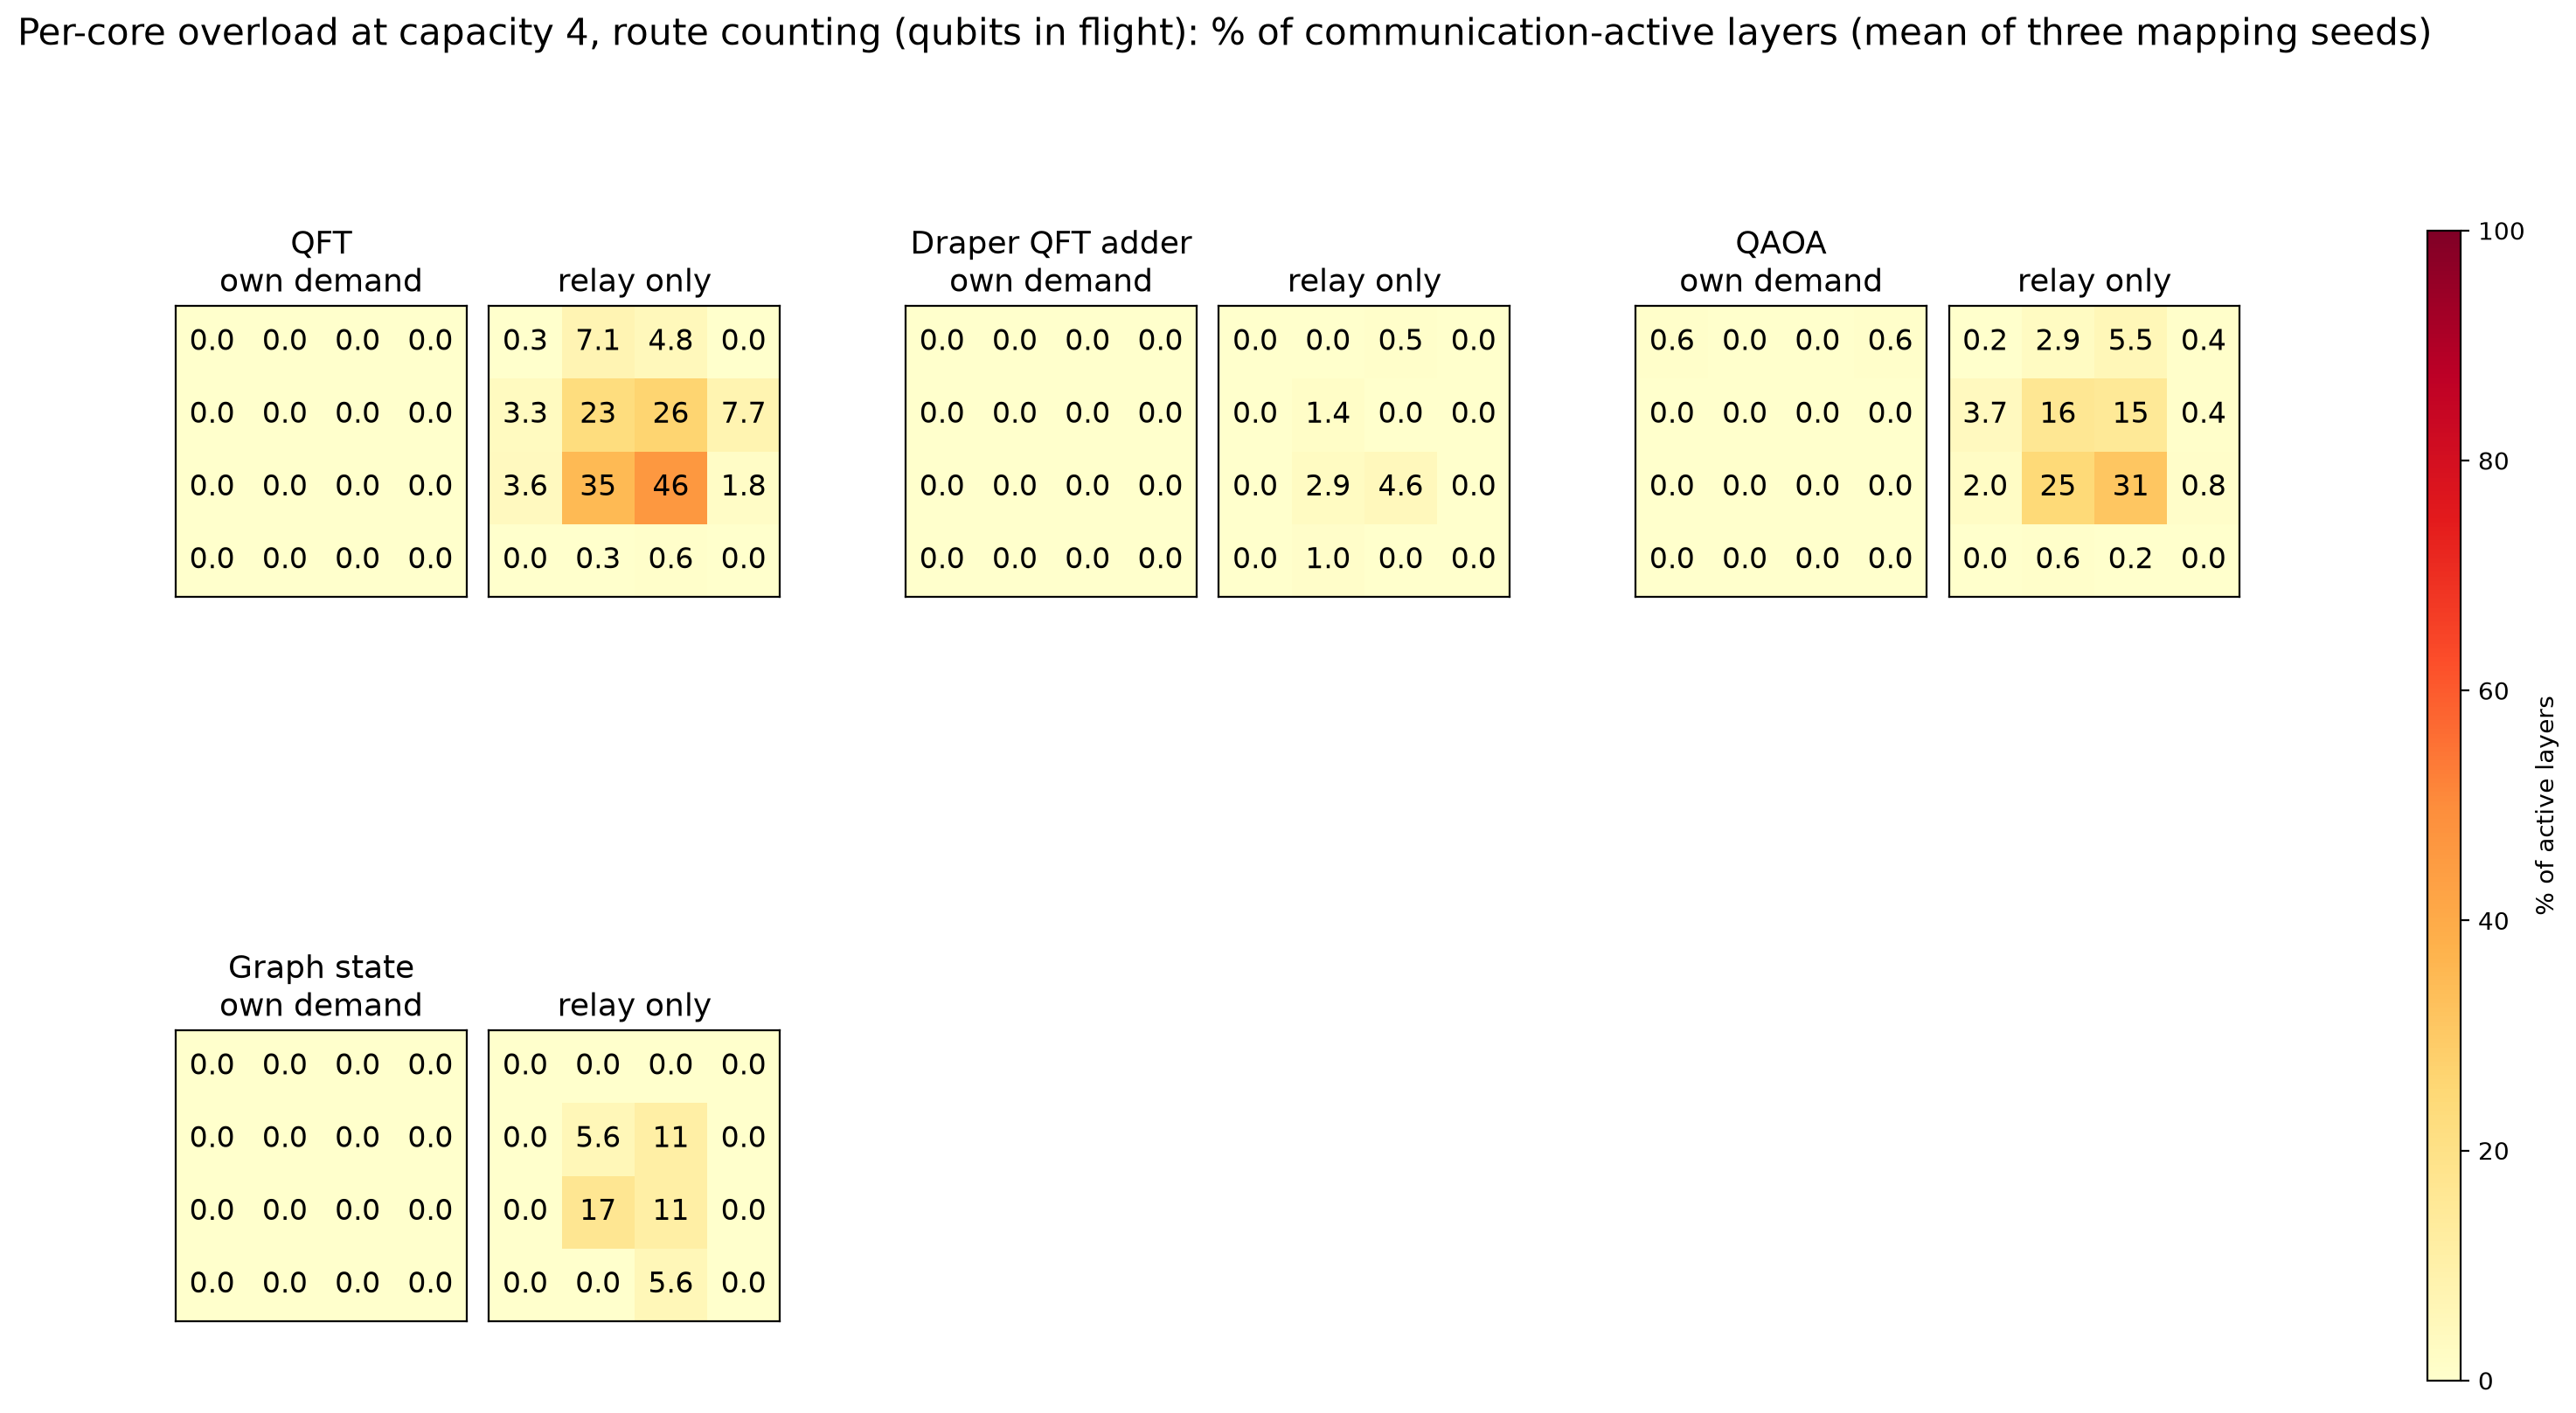
\includegraphics[width=\linewidth,height=0.80\textheight,keepaspectratio]{exp2_overview_c4_route.png}
\caption{Capacity 4, route counting (qubits in flight). For each workload with overload, the left heatmap is the percentage of its active layers in which the core is overloaded by its own endpoint demand and the right heatmap the percentage in which it is overloaded only because of relay traffic. Mesh cores are numbered row by row (core 10 is row 2, column 2). Mean of three mapping seeds.}
\label{fig:exp2-overview-c4-route}
\end{figure}
\end{landscape}
\begin{landscape}
\begin{figure}[p]
\centering
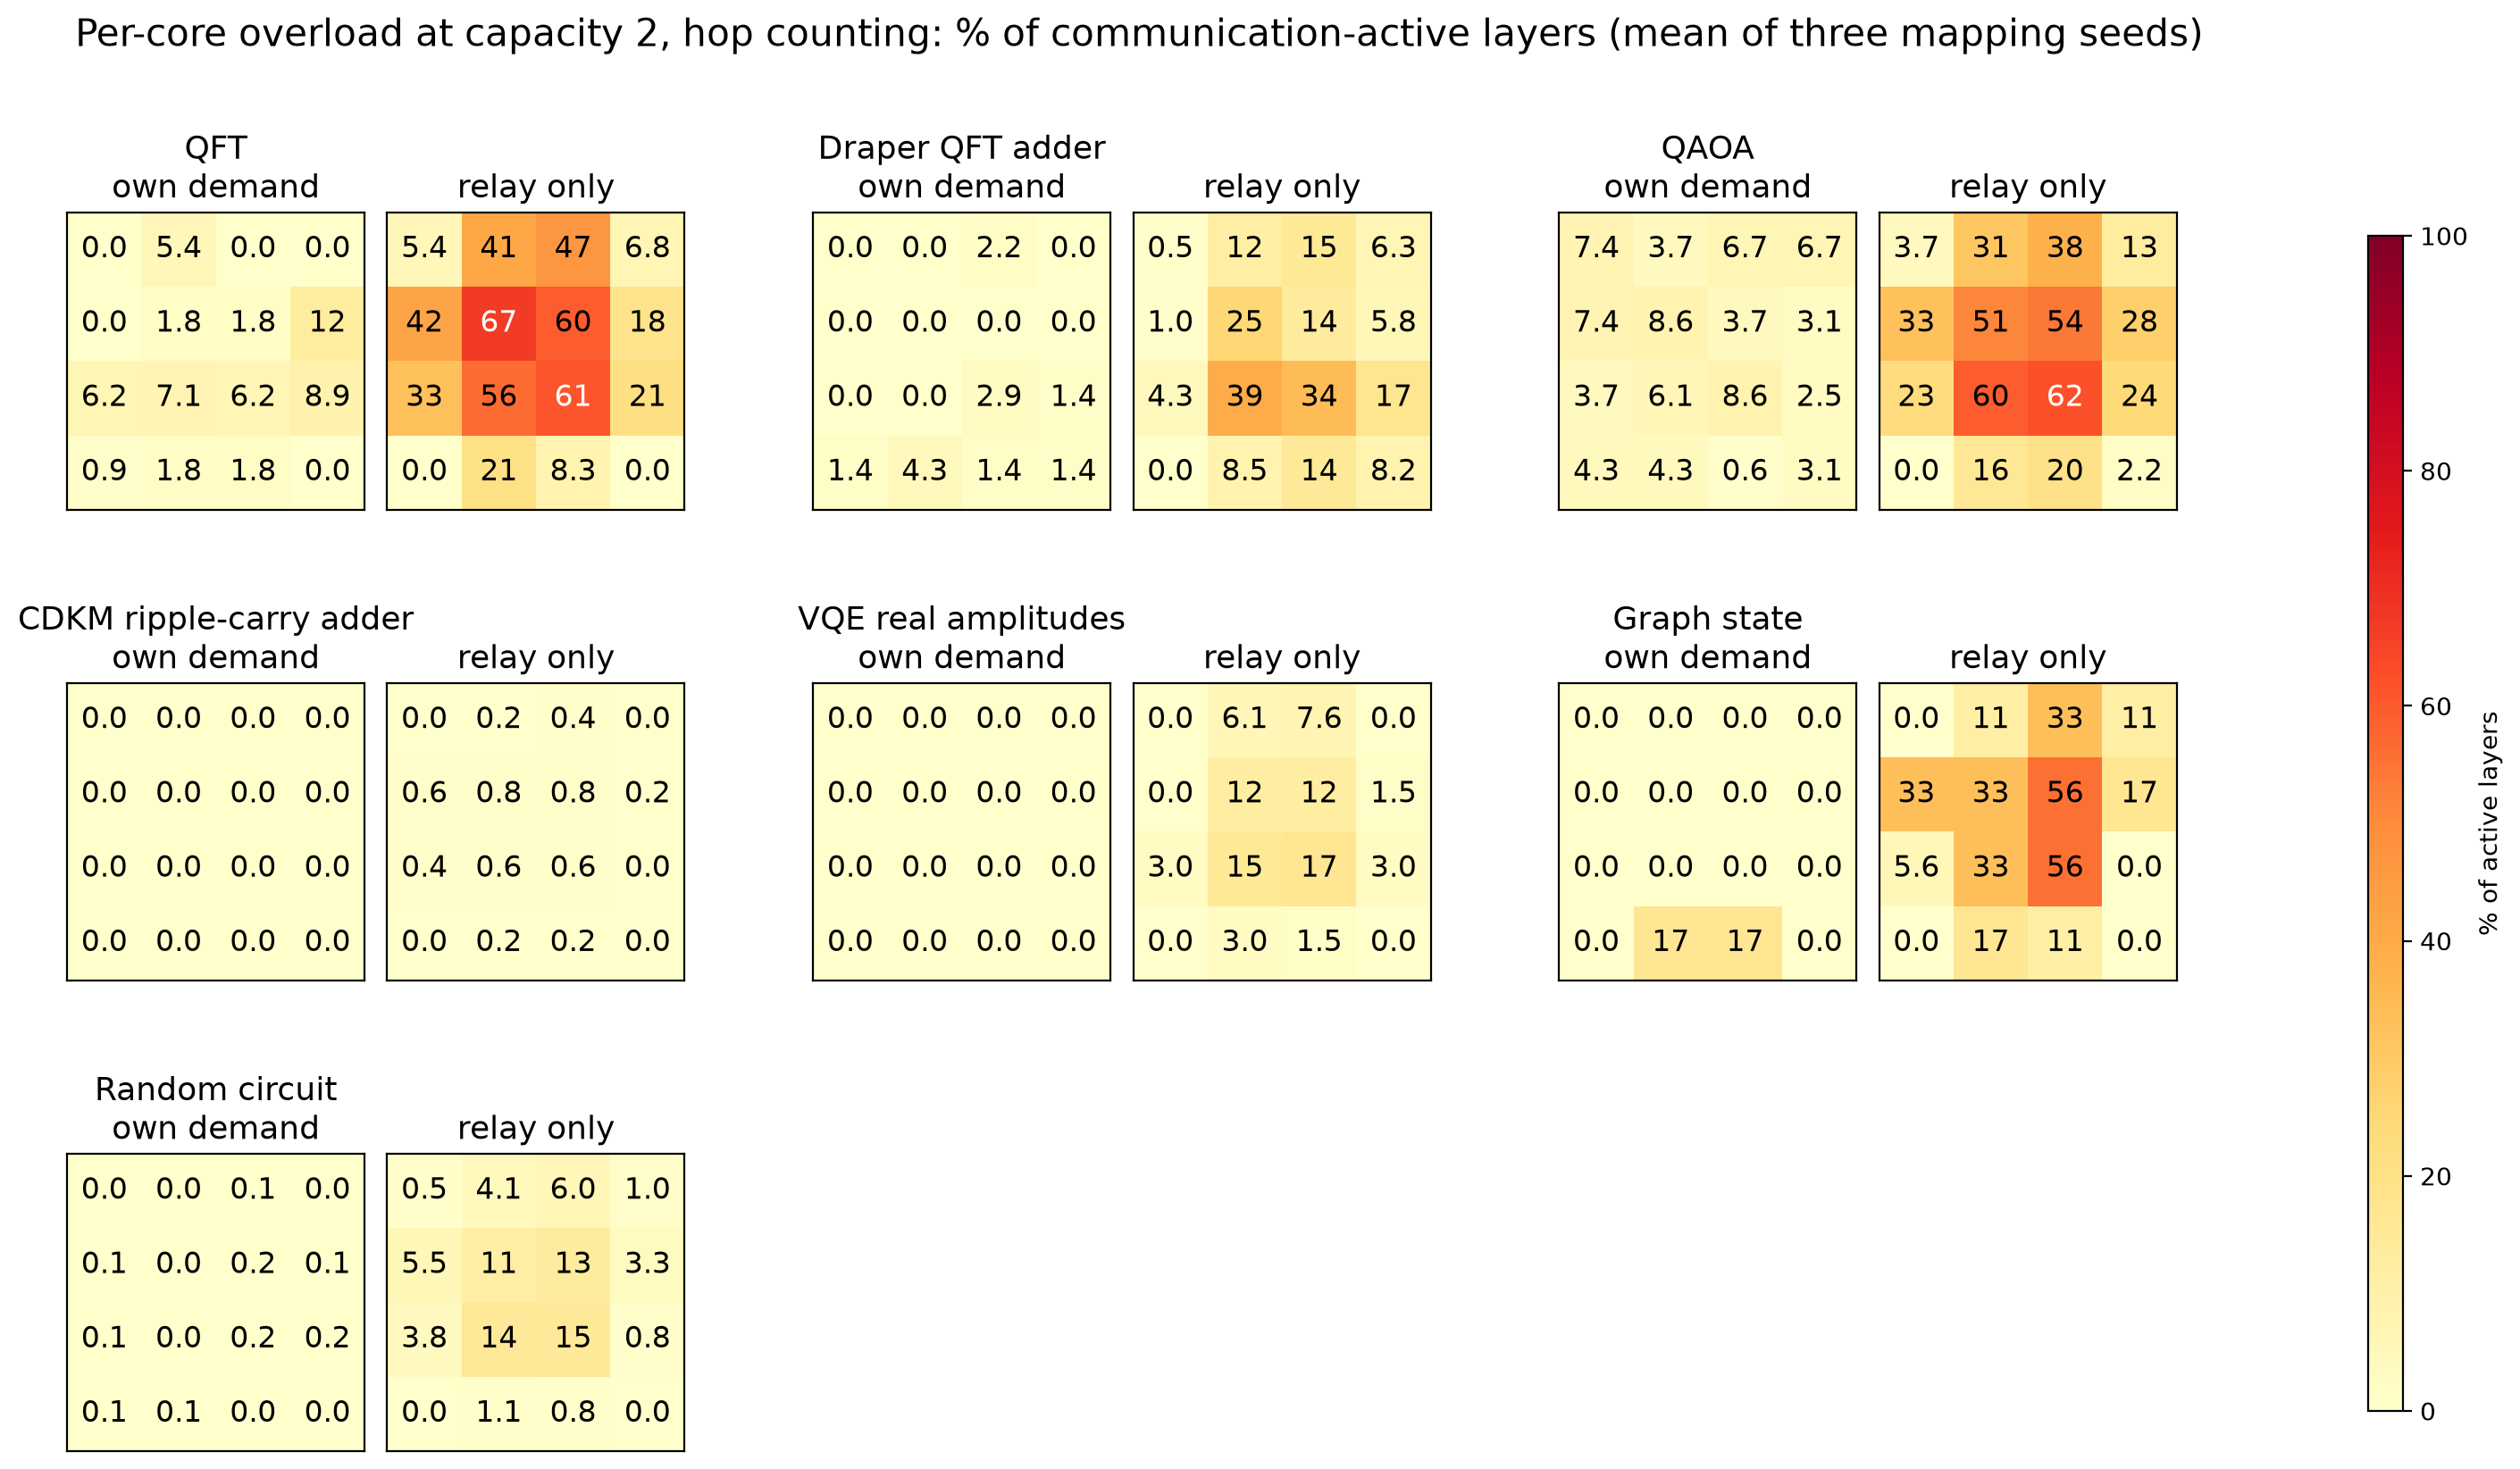
\includegraphics[width=\linewidth,height=0.80\textheight,keepaspectratio]{exp2_overview_c2_hop.png}
\caption{Capacity 2, hop counting. For each workload with overload, the left heatmap is the percentage of its active layers in which the core is overloaded by its own endpoint demand and the right heatmap the percentage in which it is overloaded only because of relay traffic. Mesh cores are numbered row by row (core 10 is row 2, column 2). Mean of three mapping seeds.}
\label{fig:exp2-overview-c2-hop}
\end{figure}
\end{landscape}
\begin{landscape}
\begin{figure}[p]
\centering
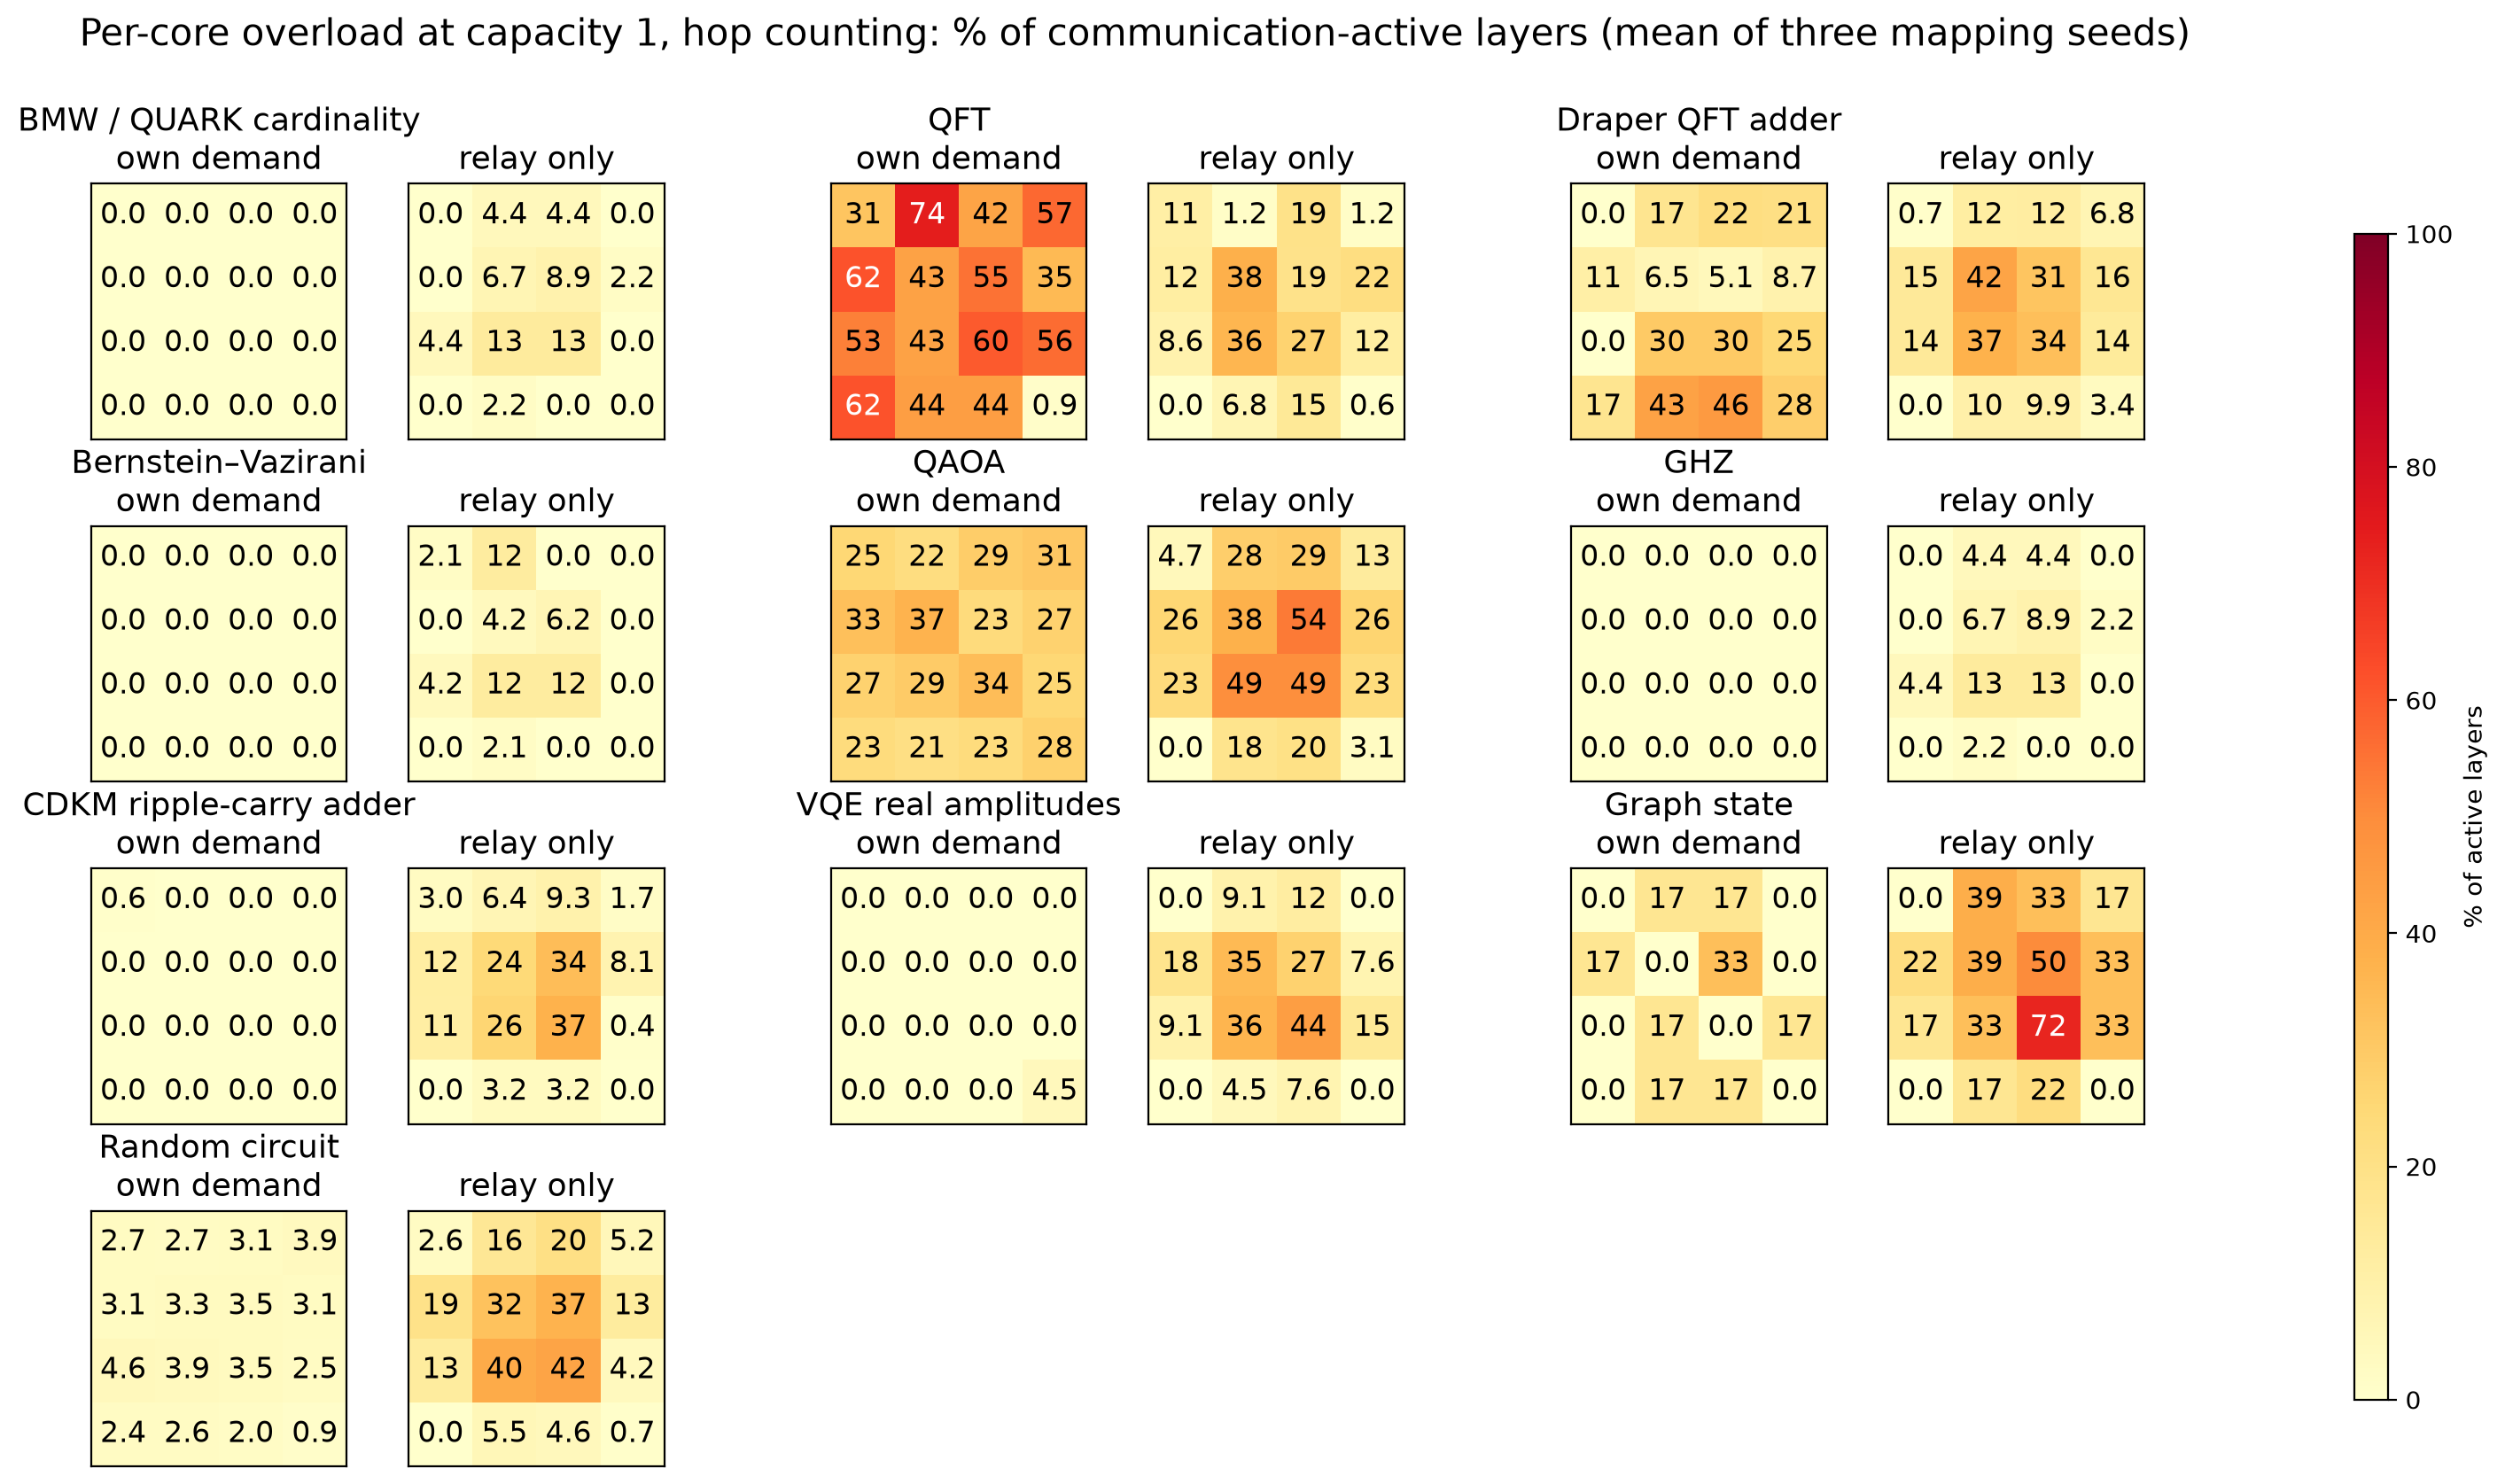
\includegraphics[width=\linewidth,height=0.80\textheight,keepaspectratio]{exp2_overview_c1_hop.png}
\caption{Capacity 1, hop counting. For each workload with overload, the left heatmap is the percentage of its active layers in which the core is overloaded by its own endpoint demand and the right heatmap the percentage in which it is overloaded only because of relay traffic. Mesh cores are numbered row by row (core 10 is row 2, column 2). Mean of three mapping seeds.}
\label{fig:exp2-overview-c1-hop}
\end{figure}
\end{landscape}
\begin{landscape}
\begin{figure}[p]
\centering
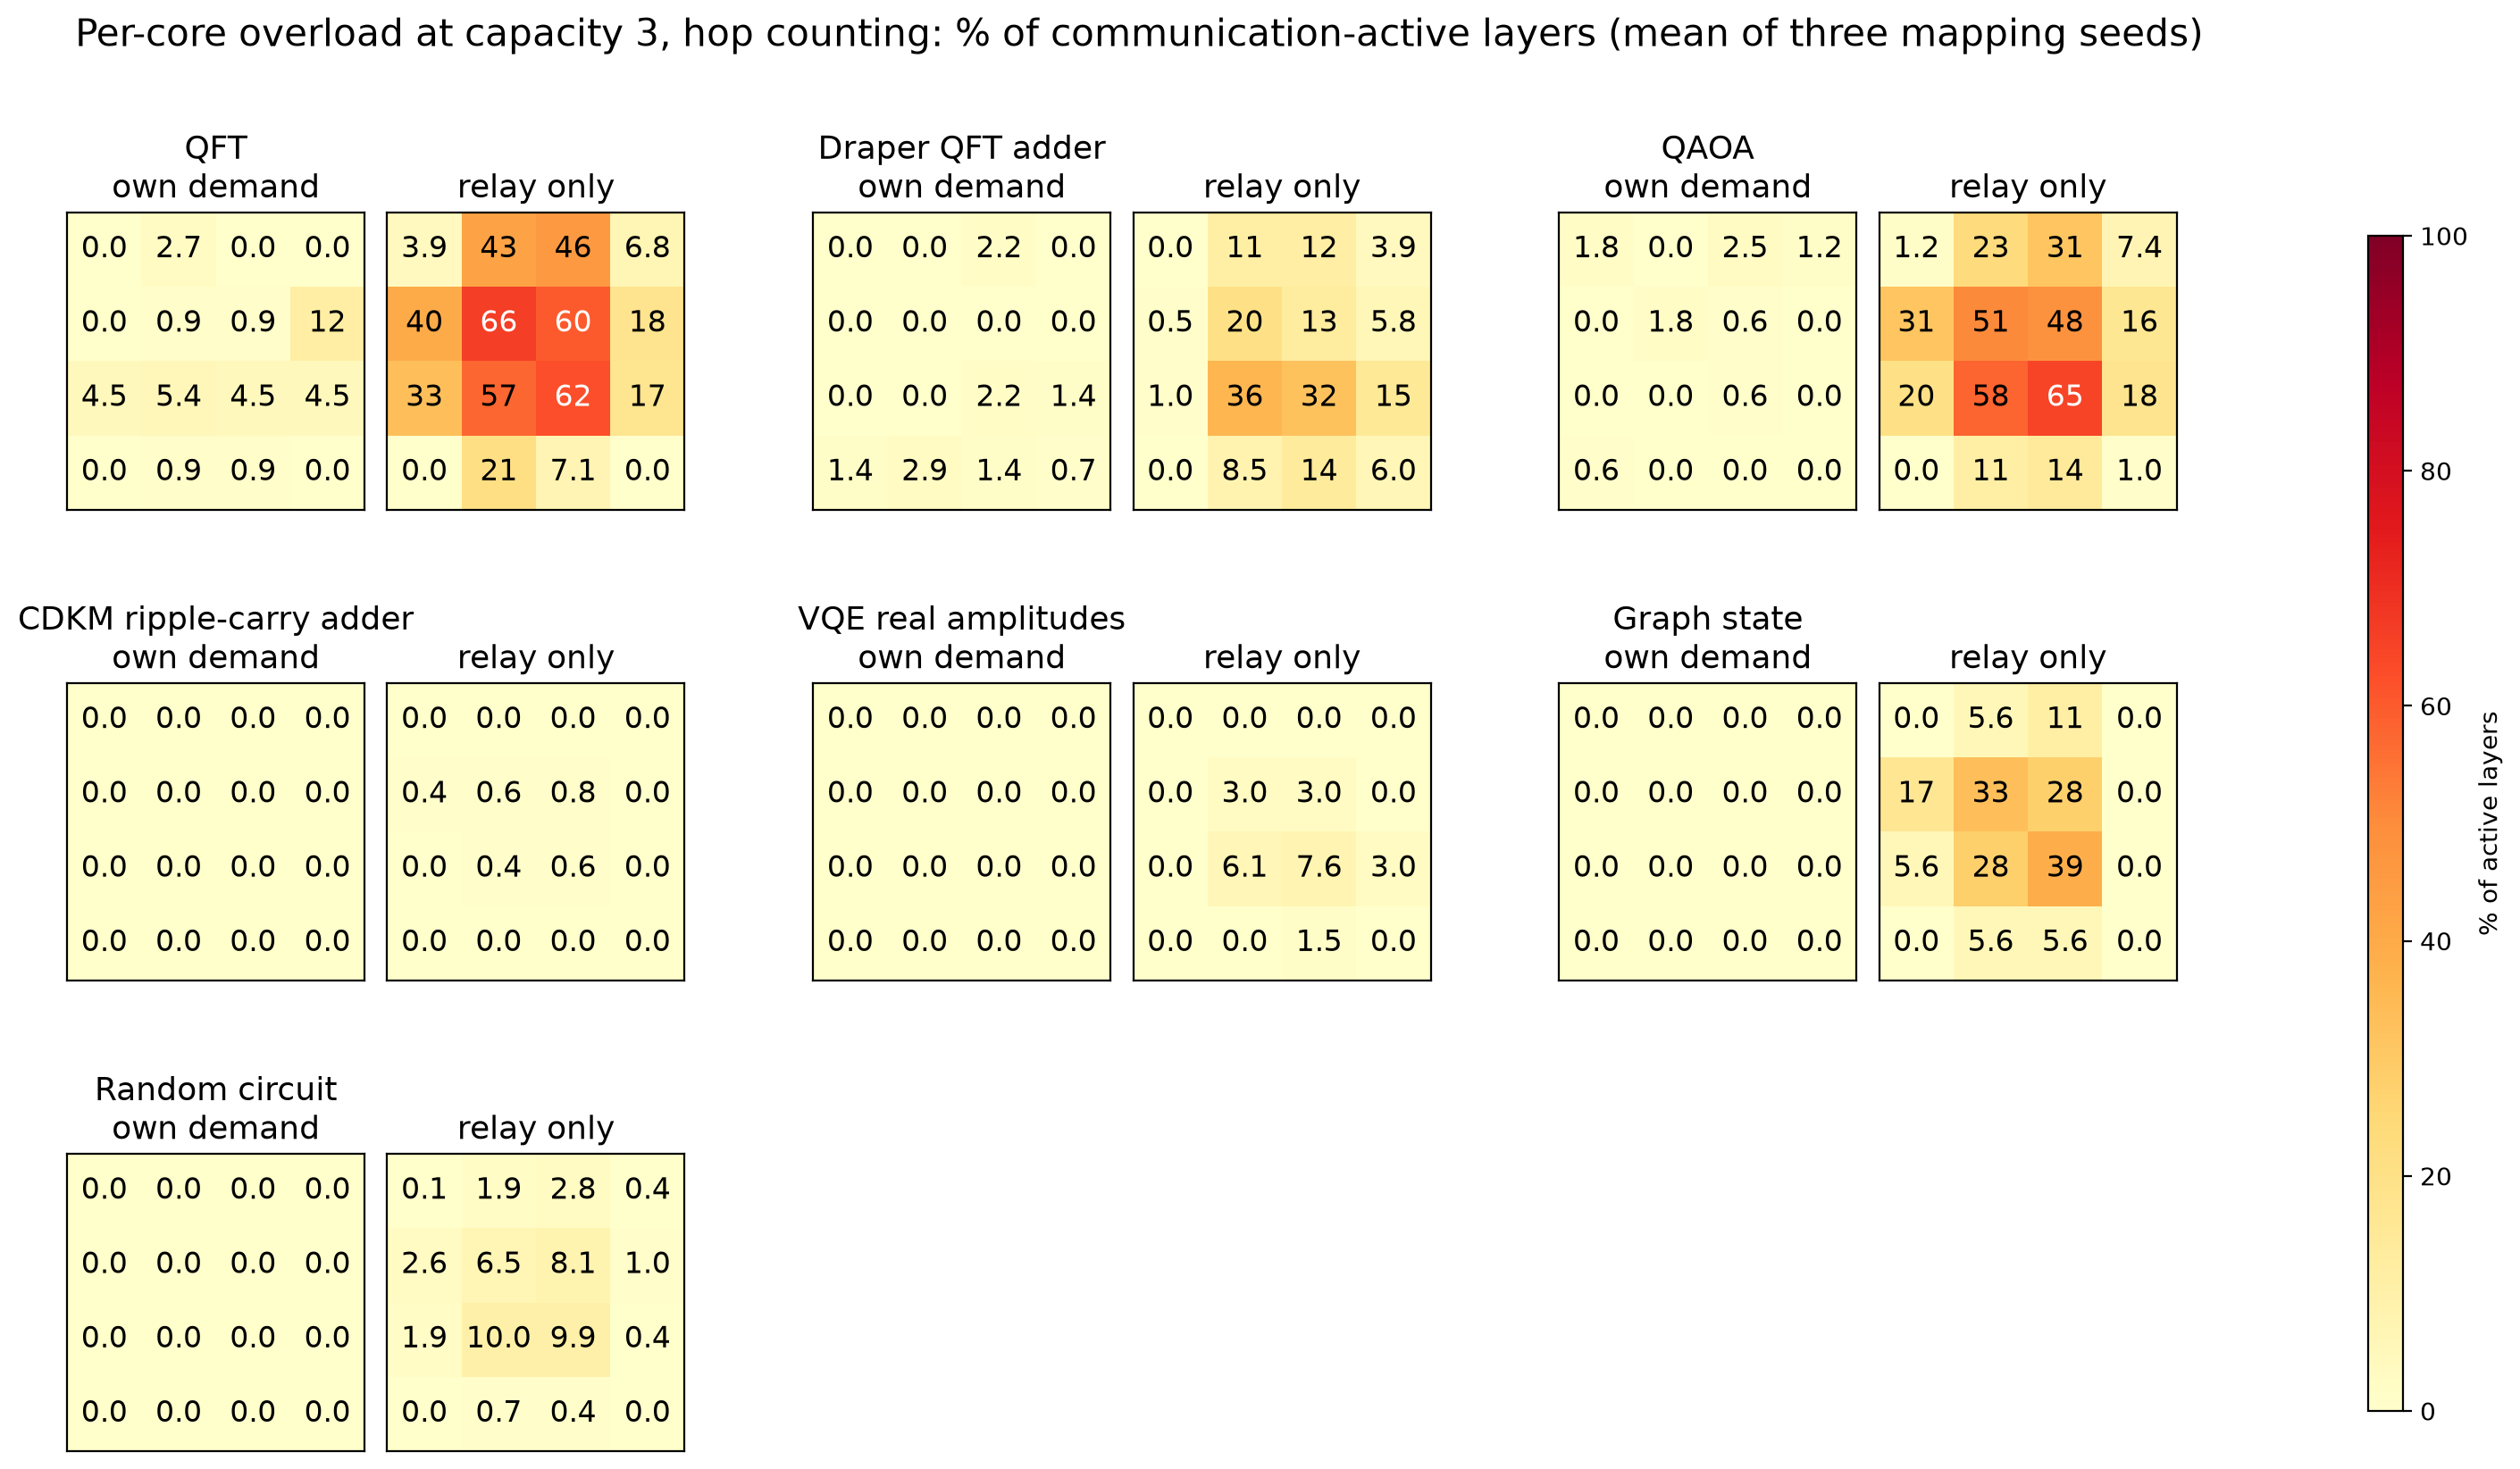
\includegraphics[width=\linewidth,height=0.80\textheight,keepaspectratio]{exp2_overview_c3_hop.png}
\caption{Capacity 3, hop counting. For each workload with overload, the left heatmap is the percentage of its active layers in which the core is overloaded by its own endpoint demand and the right heatmap the percentage in which it is overloaded only because of relay traffic. Mesh cores are numbered row by row (core 10 is row 2, column 2). Mean of three mapping seeds.}
\label{fig:exp2-overview-c3-hop}
\end{figure}
\end{landscape}
